\chapter{The Villefort Family Vault}

Two days after, a considerable crowd was assembled, towards ten o’clock
in the morning, around the door of M. de Villefort’s house, and a long
file of mourning-coaches and private carriages extended along the
Faubourg Saint-Honoré and the Rue de la Pépinière. Among them was one
of a very singular form, which appeared to have come from a distance.
It was a kind of covered wagon, painted black, and was one of the first
to arrive. Inquiry was made, and it was ascertained that, by a strange
coincidence, this carriage contained the corpse of the Marquis de
Saint-Méran, and that those who had come thinking to attend one funeral
would follow two. Their number was great. The Marquis de Saint-Méran,
one of the most zealous and faithful dignitaries of Louis XVIII. and
King Charles X., had preserved a great number of friends, and these,
added to the personages whom the usages of society gave Villefort a
claim on, formed a considerable body.

Due information was given to the authorities, and permission obtained
that the two funerals should take place at the same time. A second
hearse, decked with the same funereal pomp, was brought to M. de
Villefort’s door, and the coffin removed into it from the post-wagon.
The two bodies were to be interred in the cemetery of Père-Lachaise,
where M. de Villefort had long since had a tomb prepared for the
reception of his family. The remains of poor Renée were already
deposited there, and now, after ten years of separation, her father and
mother were to be reunited with her.

The Parisians, always curious, always affected by funereal display,
looked on with religious silence while the splendid procession
accompanied to their last abode two of the number of the old
aristocracy—the greatest protectors of commerce and sincere devotees to
their principles.

In one of the mourning-coaches Beauchamp, Debray, and Château-Renaud
were talking of the very sudden death of the marchioness.

“I saw Madame de Saint-Méran only last year at Marseilles, when I was
coming back from Algiers,” said Château-Renaud; “she looked like a
woman destined to live to be a hundred years old, from her apparent
sound health and great activity of mind and body. How old was she?”

“Franz assured me,” replied Albert, “that she was sixty-six years old.
But she has not died of old age, but of grief; it appears that since
the death of the marquis, which affected her very deeply, she has not
completely recovered her reason.”

“But of what disease, then, did she die?” asked Debray.

“It is said to have been a congestion of the brain, or apoplexy, which
is the same thing, is it not?”

“Nearly.”

“It is difficult to believe that it was apoplexy,” said Beauchamp.
“Madame de Saint-Méran, whom I once saw, was short, of slender form,
and of a much more nervous than sanguine temperament; grief could
hardly produce apoplexy in such a constitution as that of Madame de
Saint-Méran.”

“At any rate,” said Albert, “whatever disease or doctor may have killed
her, M. de Villefort, or rather, Mademoiselle Valentine,—or, still
rather, our friend Franz, inherits a magnificent fortune, amounting, I
believe, to 80,000 livres per annum.”

“And this fortune will be doubled at the death of the old Jacobin,
Noirtier.”

“That is a tenacious old grandfather,” said Beauchamp. “\textit{Tenacem
propositi virum}. I think he must have made an agreement with death to
outlive all his heirs, and he appears likely to succeed. He resembles
the old Conventionalist of ’93, who said to Napoleon, in 1814, ‘You
bend because your empire is a young stem, weakened by rapid growth.
Take the Republic for a tutor; let us return with renewed strength to
the battle-field, and I promise you 500,000 soldiers, another Marengo,
and a second Austerlitz. Ideas do not become extinct, sire; they
slumber sometimes, but only revive the stronger before they sleep
entirely.’”

“Ideas and men appeared the same to him,” said Albert. “One thing only
puzzles me, namely, how Franz d’Épinay will like a grandfather who
cannot be separated from his wife. But where is Franz?”

“In the first carriage, with M. de Villefort, who considers him already
as one of the family.”

\begin{figure}[ht]
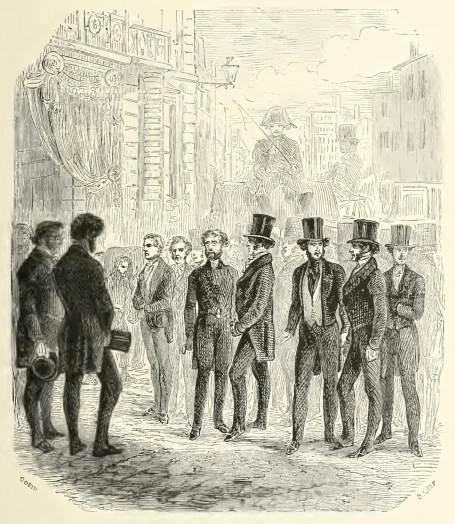
\includegraphics[width=\textwidth]{40024m.jpg}
\end{figure}

Such was the conversation in almost all the carriages; these two sudden
deaths, so quickly following each other, astonished everyone, but no
one suspected the terrible secret which M. d’Avrigny had communicated,
in his nocturnal walk to M. de Villefort. They arrived in about an hour
at the cemetery; the weather was mild, but dull, and in harmony with
the funeral ceremony. Among the groups which flocked towards the family
vault, Château-Renaud recognized Morrel, who had come alone in a
cabriolet, and walked silently along the path bordered with yew-trees.

“You here?” said Château-Renaud, passing his arms through the young
captain’s; “are you a friend of Villefort’s? How is it that I have
never met you at his house?”

“I am no acquaintance of M. de Villefort’s,” answered Morrel, “but I
was of Madame de Saint-Méran.” Albert came up to them at this moment
with Franz.

“The time and place are but ill-suited for an introduction.” said
Albert; “but we are not superstitious. M. Morrel, allow me to present
to you M. Franz d’Épinay, a delightful travelling companion, with whom
I made the tour of Italy. My dear Franz, M. Maximilian Morrel, an
excellent friend I have acquired in your absence, and whose name you
will hear me mention every time I make any allusion to affection, wit,
or amiability.”

Morrel hesitated for a moment; he feared it would be hypocritical to
accost in a friendly manner the man whom he was tacitly opposing, but
his oath and the gravity of the circumstances recurred to his memory;
he struggled to conceal his emotion and bowed to Franz.

“Mademoiselle de Villefort is in deep sorrow, is she not?” said Debray
to Franz.

“Extremely,” replied he; “she looked so pale this morning, I scarcely
knew her.”

These apparently simple words pierced Morrel to the heart. This man had
seen Valentine, and spoken to her! The young and high-spirited officer
required all his strength of mind to resist breaking his oath. He took
the arm of Château-Renaud, and turned towards the vault, where the
attendants had already placed the two coffins.

“This is a magnificent habitation,” said Beauchamp, looking towards the
mausoleum; “a summer and winter palace. You will, in turn, enter it, my
dear d’Épinay, for you will soon be numbered as one of the family. I,
as a philosopher, should like a little country-house, a cottage down
there under the trees, without so many free-stones over my poor body.
In dying, I will say to those around me what Voltaire wrote to Piron:
‘\textit{Eo rus}, and all will be over.’ But come, Franz, take courage, your
wife is an heiress.”

“Indeed, Beauchamp, you are unbearable. Politics has made you laugh at
everything, and political men have made you disbelieve everything. But
when you have the honor of associating with ordinary men, and the
pleasure of leaving politics for a moment, try to find your
affectionate heart, which you leave with your stick when you go to the
Chamber.”

“But tell me,” said Beauchamp, “what is life? Is it not a halt in
Death’s anteroom?”

\begin{figure}[ht]
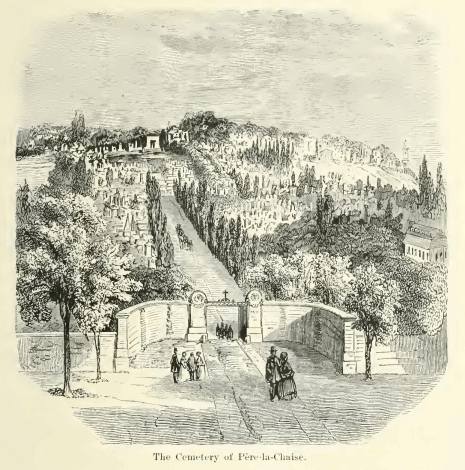
\includegraphics[width=\textwidth]{40026m.jpg}
\end{figure}

“I am prejudiced against Beauchamp,” said Albert, drawing Franz away,
and leaving the former to finish his philosophical dissertation with
Debray.

The Villefort vault formed a square of white stones, about twenty feet
high; an interior partition separated the two families, and each
apartment had its entrance door. Here were not, as in other tombs,
ignoble drawers, one above another, where thrift bestows its dead and
labels them like specimens in a museum; all that was visible within the
bronze gates was a gloomy-looking room, separated by a wall from the
vault itself. The two doors before mentioned were in the middle of this
wall, and enclosed the Villefort and Saint-Méran coffins. There grief
might freely expend itself without being disturbed by the trifling
loungers who came from a picnic party to visit Père-Lachaise, or by
lovers who make it their rendezvous.

The two coffins were placed on trestles previously prepared for their
reception in the right-hand crypt belonging to the Saint-Méran family.
Villefort, Franz, and a few near relatives alone entered the sanctuary.

As the religious ceremonies had all been performed at the door, and
there was no address given, the party all separated; Château-Renaud,
Albert, and Morrel, went one way, and Debray and Beauchamp the other.
Franz remained with M. de Villefort; at the gate of the cemetery Morrel
made an excuse to wait; he saw Franz and M. de Villefort get into the
same mourning-coach, and thought this meeting forboded evil. He then
returned to Paris, and although in the same carriage with
Château-Renaud and Albert, he did not hear one word of their
conversation.

As Franz was about to take leave of M. de Villefort, “When shall I see
you again?” said the latter.

“At what time you please, sir,” replied Franz.

“As soon as possible.”

“I am at your command, sir; shall we return together?”

“If not unpleasant to you.”

“On the contrary, I shall feel much pleasure.”

Thus, the future father and son-in-law stepped into the same carriage,
and Morrel, seeing them pass, became uneasy. Villefort and Franz
returned to the Faubourg Saint-Honoré. The procureur, without going to
see either his wife or his daughter, went at once to his study, and,
offering the young man a chair:

“M. d’Épinay,” said he, “allow me to remind you at this moment,—which
is perhaps not so ill-chosen as at first sight may appear, for
obedience to the wishes of the departed is the first offering which
should be made at their tomb,—allow me then to remind you of the wish
expressed by Madame de Saint-Méran on her death-bed, that Valentine’s
wedding might not be deferred. You know the affairs of the deceased are
in perfect order, and her will bequeaths to Valentine the entire
property of the Saint-Méran family; the notary showed me the documents
yesterday, which will enable us to draw up the contract immediately.
You may call on the notary, M. Deschamps, Place Beauveau, Faubourg
Saint-Honoré, and you have my authority to inspect those deeds.”

“Sir,” replied M. d’Épinay, “it is not, perhaps, the moment for
Mademoiselle Valentine, who is in deep distress, to think of a husband;
indeed, I fear——”

\begin{figure}[ht]
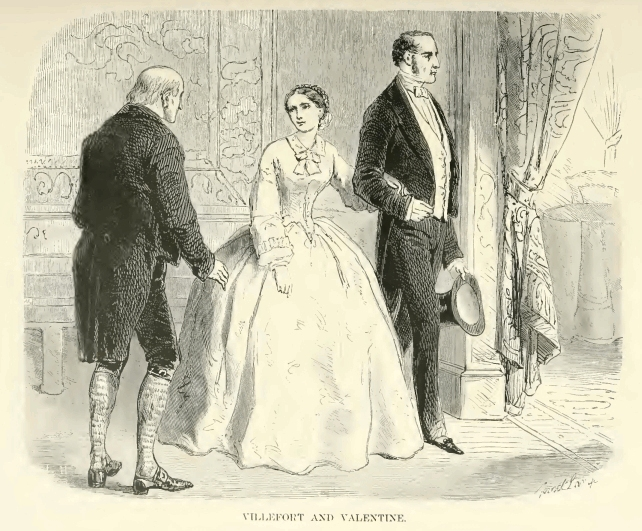
\includegraphics[width=\textwidth]{40028m.jpg}
\end{figure}

“Valentine will have no greater pleasure than that of fulfilling her
grandmother’s last injunctions; there will be no obstacle from that
quarter, I assure you.”

“In that case,” replied Franz, “as I shall raise none, you may make
arrangements when you please; I have pledged my word, and shall feel
pleasure and happiness in adhering to it.”

“Then,” said Villefort, “nothing further is required. The contract was
to have been signed three days since; we shall find it all ready, and
can sign it today.”

“But the mourning?” said Franz, hesitating.

“Don’t be uneasy on that score,” replied Villefort; “no ceremony will
be neglected in my house. Mademoiselle de Villefort may retire during
the prescribed three months to her estate of Saint-Méran; I say hers,
for she inherits it today. There, after a few days, if you like, the
civil marriage shall be celebrated without pomp or ceremony. Madame de
Saint-Méran wished her daughter should be married there. When that is
over, you, sir, can return to Paris, while your wife passes the time of
her mourning with her mother-in-law.”

“As you please, sir,” said Franz.

“Then,” replied M. de Villefort, “have the kindness to wait half an
hour; Valentine shall come down into the drawing-room. I will send for
M. Deschamps; we will read and sign the contract before we separate,
and this evening Madame de Villefort shall accompany Valentine to her
estate, where we will rejoin them in a week.”

“Sir,” said Franz, “I have one request to make.”

“What is it?”

“I wish Albert de Morcerf and Raoul de Château-Renaud to be present at
this signature; you know they are my witnesses.”

“Half an hour will suffice to apprise them; will you go for them
yourself, or shall you send?”

“I prefer going, sir.”

“I shall expect you, then, in half an hour, baron, and Valentine will
be ready.”

Franz bowed and left the room. Scarcely had the door closed, when M. de
Villefort sent to tell Valentine to be ready in the drawing-room in
half an hour, as he expected the notary and M. d’Épinay and his
witnesses. The news caused a great sensation throughout the house;
Madame de Villefort would not believe it, and Valentine was
thunderstruck. She looked around for help, and would have gone down to
her grandfather’s room, but on the stairs she met M. de Villefort, who
took her arm and led her into the drawing-room. In the anteroom,
Valentine met Barrois, and looked despairingly at the old servant. A
moment later, Madame de Villefort entered the drawing-room with her
little Edward. It was evident that she had shared the grief of the
family, for she was pale and looked fatigued. She sat down, took Edward
on her knees, and from time to time pressed this child, on whom her
affections appeared centred, almost convulsively to her bosom.

Two carriages were soon heard to enter the courtyard. One was the
notary’s; the other, that of Franz and his friends. In a moment the
whole party was assembled. Valentine was so pale one might trace the
blue veins from her temples, round her eyes and down her cheeks. Franz
was deeply affected. Château-Renaud and Albert looked at each other
with amazement; the ceremony which was just concluded had not appeared
more sorrowful than did that which was about to begin. Madame de
Villefort had placed herself in the shadow behind a velvet curtain, and
as she constantly bent over her child, it was difficult to read the
expression of her face. M. de Villefort was, as usual, unmoved.

The notary, after having, according to the customary method, arranged
the papers on the table, taken his place in an armchair, and raised his
spectacles, turned towards Franz:

“Are you M. Franz de Quesnel, baron d’Épinay?” asked he, although he
knew it perfectly.

“Yes, sir,” replied Franz. The notary bowed.

“I have, then, to inform you, sir, at the request of M. de Villefort,
that your projected marriage with Mademoiselle de Villefort has changed
the feeling of M. Noirtier towards his grandchild, and that he
disinherits her entirely of the fortune he would have left her. Let me
hasten to add,” continued he, “that the testator, having only the right
to alienate a part of his fortune, and having alienated it all, the
will will not bear scrutiny, and is declared null and void.”

“Yes.” said Villefort; “but I warn M. d’Épinay, that during my
life-time my father’s will shall never be questioned, my position
forbidding any doubt to be entertained.”

\begin{figure}[ht]
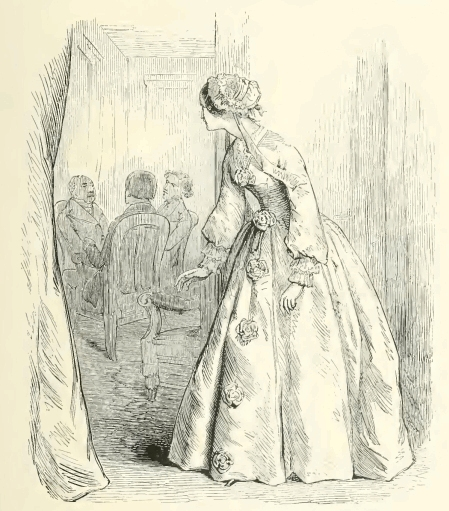
\includegraphics[width=\textwidth]{40032m.jpg}
\end{figure}

“Sir,” said Franz, “I regret much that such a question has been raised
in the presence of Mademoiselle Valentine; I have never inquired the
amount of her fortune, which, however limited it may be, exceeds mine.
My family has sought consideration in this alliance with M. de
Villefort; all I seek is happiness.”

Valentine imperceptibly thanked him, while two silent tears rolled down
her cheeks.

“Besides, sir,” said Villefort, addressing himself to his future
son-in-law, “excepting the loss of a portion of your hopes, this
unexpected will need not personally wound you; M. Noirtier’s weakness
of mind sufficiently explains it. It is not because Mademoiselle
Valentine is going to marry you that he is angry, but because she will
marry, a union with any other would have caused him the same sorrow.
Old age is selfish, sir, and Mademoiselle de Villefort has been a
faithful companion to M. Noirtier, which she cannot be when she becomes
the Baroness d’Épinay. My father’s melancholy state prevents our
speaking to him on any subjects, which the weakness of his mind would
incapacitate him from understanding, and I am perfectly convinced that
at the present time, although, he knows that his granddaughter is going
to be married, M. Noirtier has even forgotten the name of his intended
grandson.” M. de Villefort had scarcely said this, when the door
opened, and Barrois appeared.

“Gentlemen,” said he, in a tone strangely firm for a servant speaking
to his masters under such solemn circumstances,—“gentlemen, M. Noirtier
de Villefort wishes to speak immediately to M. Franz de Quesnel, baron
d’Épinay.” He, as well as the notary, that there might be no mistake in
the person, gave all his titles to the bridegroom elect.

Villefort started, Madame de Villefort let her son slip from her knees,
Valentine rose, pale and dumb as a statue. Albert and Château-Renaud
exchanged a second look, more full of amazement than the first. The
notary looked at Villefort.

“It is impossible,” said the procureur. “M. d’Épinay cannot leave the
drawing-room at present.”

“It is at this moment,” replied Barrois with the same firmness, “that
M. Noirtier, my master, wishes to speak on important subjects to M.
Franz d’Épinay.”

“Grandpapa Noirtier can speak now, then,” said Edward, with his
habitual quickness. However, his remark did not make Madame de
Villefort even smile, so much was every mind engaged, and so solemn was
the situation.

“Tell M. Nortier,” resumed Villefort, “that what he demands is
impossible.”

“Then, M. Nortier gives notice to these gentlemen,” replied Barrois,
“that he will give orders to be carried to the drawing-room.”

Astonishment was at its height. Something like a smile was perceptible
on Madame de Villefort’s countenance. Valentine instinctively raised
her eyes, as if to thank heaven.

“Pray go, Valentine,” said; M. de Villefort, “and see what this new
fancy of your grandfather’s is.” Valentine rose quickly, and was
hastening joyfully towards the door, when M. de Villefort altered his
intention.

“Stop,” said he; “I will go with you.”

“Excuse me, sir,” said Franz, “since M. Noirtier sent for me, I am
ready to attend to his wish; besides, I shall be happy to pay my
respects to him, not having yet had the honor of doing so.”

“Pray, sir,” said Villefort with marked uneasiness, “do not disturb
yourself.”

\begin{figure}[ht]
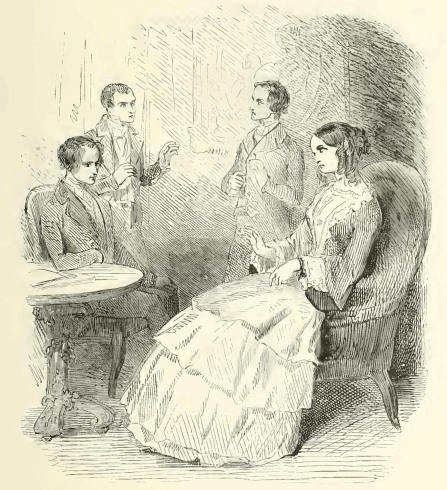
\includegraphics[width=\textwidth]{40034m.jpg}
\end{figure}

“Forgive me, sir,” said Franz in a resolute tone. “I would not lose
this opportunity of proving to M. Noirtier how wrong it would be of him
to encourage feelings of dislike to me, which I am determined to
conquer, whatever they may be, by my devotion.”

And without listening to Villefort he arose, and followed Valentine,
who was running downstairs with the joy of a shipwrecked mariner who
finds a rock to cling to. M. de Villefort followed them. Château-Renaud
and Morcerf exchanged a third look of still increasing wonder.
